\section{Use SFTP to Transfer Code to Raspberry Pi}
\label{use_sftp_transfer_code_raspberrypi}

Secure File Transfer Protocol (SFTP), lets you transfer files from a computer to a Pi. SFTP uses SSH to
copy files to and from the Raspberry Pi over the network. Let's see how this works with a simple
example. Create the following script in a directory on your PC that you will be storing the code
of your robot.

\begin{lstlisting}
## sftp_test.py
print("SFTP transfer example")
\end{lstlisting}

We can use the SFTP tool FileZilla. You can download FileZilla from here \url{https:/​/​filezilla-​project.​org} 

Plug in and power up your Raspberry Pi. Whether you are connected or not is shown  in the bottom of the right-hand panel.
In the \textbf{Host} box, type the local hostname you gave your robot Pi when you did the headless setup, prefixed with \url{sftp://}. 
For example, \url{sftp://raspberrypi.local}. In the \textbf{Username}, type \lstinline{pi} and enter the password you set up before. Click the 
\textbf{Quickconnect} button to connect to the Raspberry Pi. Figure \ref{raspberrypi_sftp} shows a connected session with
our \lstinline{sftp_test.py} file transferred across.

\begin{figure}[!htb]
\begin{center}
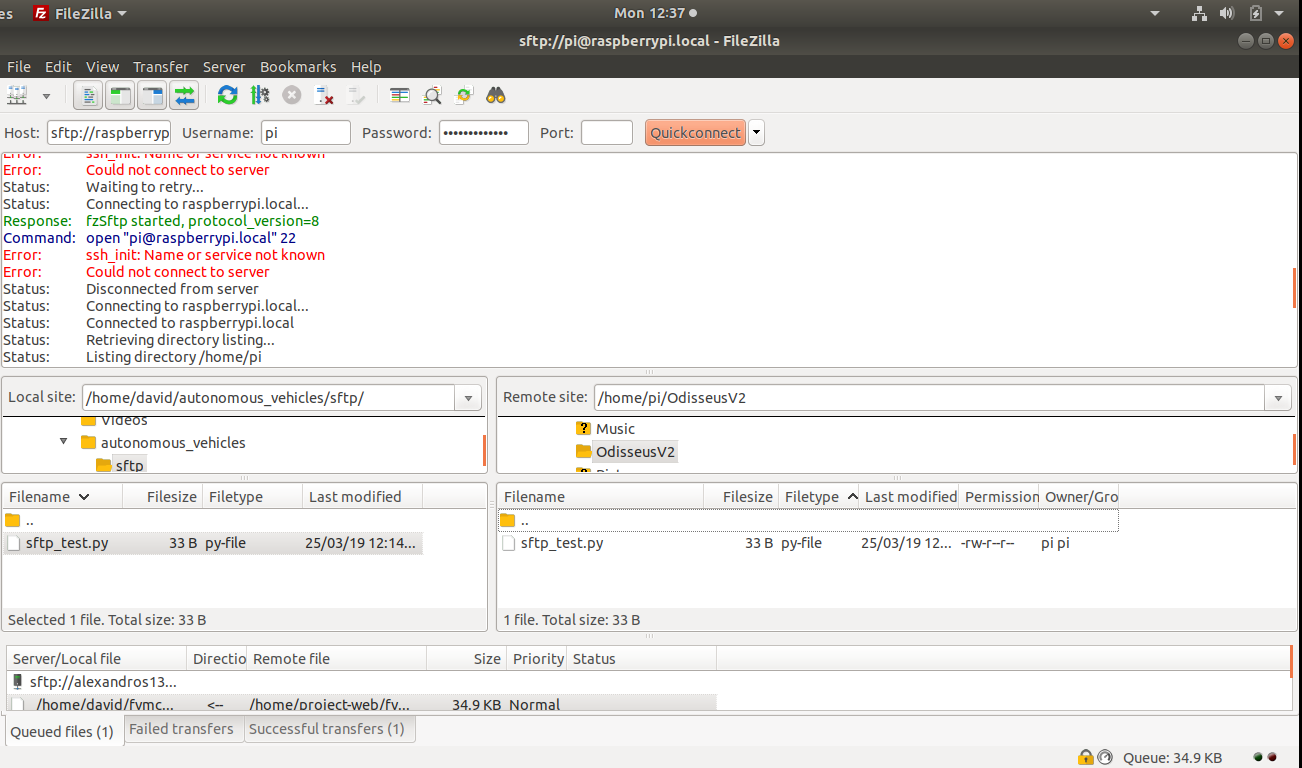
\includegraphics[scale=0.280]{img/raspberrypi/sftp.png}
\end{center}
\caption{GUI view of FileZilla.}
\label{raspberrypi_sftp}
\end{figure}

When connected, you will see files on the Raspberry Pi in the right-hand \textbf{Remote site} panel,
like the preceding image. Use the left-hand \textbf{Local site} panel to go to your code on your
computer. You can click \lstinline{sftp_test.py} and drag it to the the lower right-hand panel to put it on the Raspberry Pi.


When you drag the file over, you should see it in the \textbf{Queued files} section (left bottom corner). Since this file is
small, it will only be in this queued state for an instant. You can also use the same system
too for larger files and folders. You'll soon see the file over in the remote site (the Raspberry Pi), shown on the right of the preceding screenshot. 
To run this code, use PuTTY to log in to the Pi. This is shown in Figure \ref{raspberrypi_putty_session}:




\begin{figure}[!htb]
\begin{center}
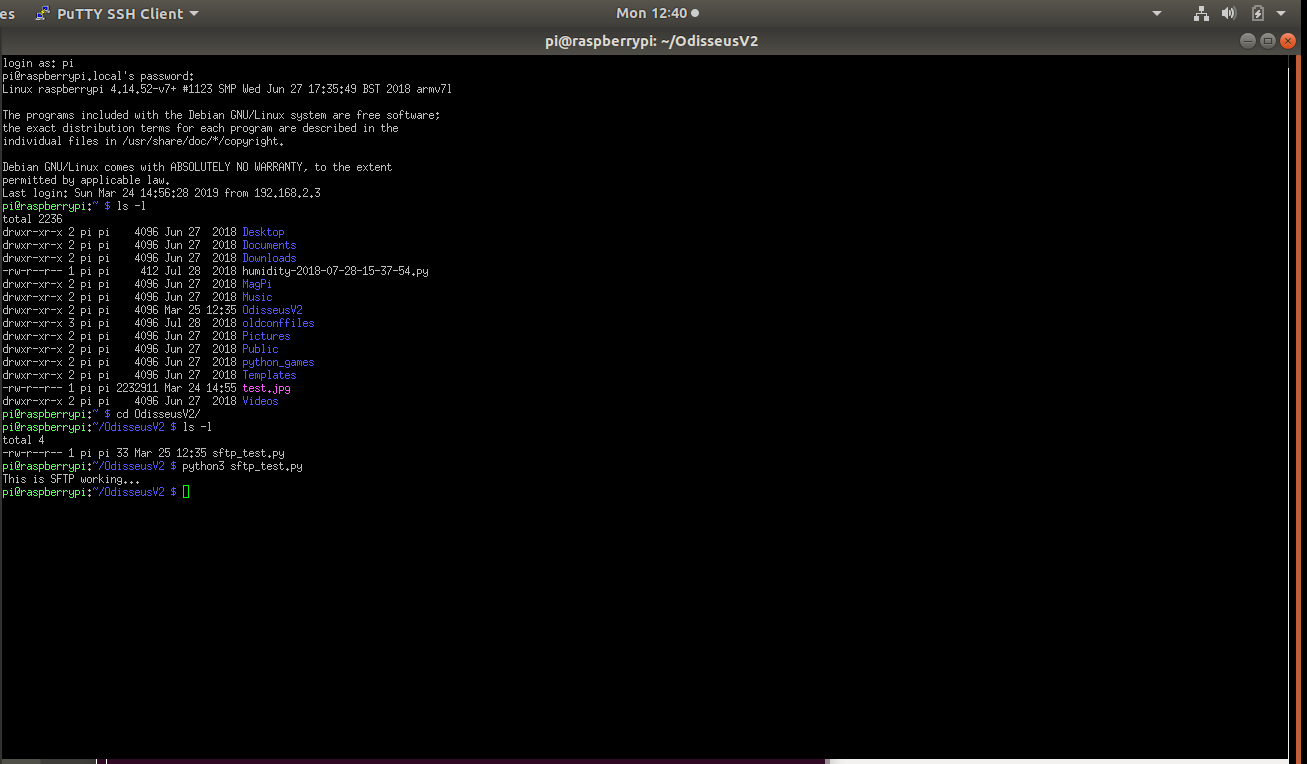
\includegraphics[scale=0.280]{img/raspberrypi/putty.png}
\end{center}
\caption{RaspberryPi PuTTY session.}
\label{raspberrypi_putty_session}
\end{figure}


